\documentclass[10pt,twocolumn,letterpaper]{article}
\usepackage[review]{cvpr}
% Additional packages; loaded before hyperref (see main.tex), as required by the CVPR 2027 author kit.
\usepackage{graphicx}
\usepackage{amsmath,amssymb}
\usepackage{booktabs}
\newcommand{\paperTitle}{High-Reach Candidate Search for Longitudinal Lung Lesion Matching}

\newcommand{\pp}{\,\mathrm{pp}}
% ---- added in revision ----
\usepackage{cuted}           % page-1 teaser strip
\usepackage{caption}
\usepackage{multirow}
\usepackage{algorithm}
\usepackage[noend]{algpseudocode}
\usepackage{xspace}
\newcommand{\TODO}[1]{\textbf{\color{red}[TODO: #1]}}
% \renewcommand{\TODO}[1]{}  % uncomment before submission
\DeclareMathOperator*{\argmax}{arg\,max}
\newcommand{\ours}{Diverse search\xspace}
\newcommand{\T}{\mathcal{T}}   % translation lattice
\newcommand{\Ss}{\mathcal{S}}  % retained (diversified) set
\usepackage{placeins}

\renewcommand{\thesection}{S\arabic{section}}
\renewcommand{\thetable}{S\arabic{table}}
\renewcommand{\thefigure}{S\arabic{figure}}
\title{\paperTitle\\[0.25em]\large Supplementary Material}
\author{Anonymous CVPR submission}
\hypersetup{pdftitle={\paperTitle\ - Supplement}}

\begin{document}
\maketitle

\section{Cohorts and analysis conventions}
\begin{table}[t]
\centering\small
\caption{Archived LUNA25 flow. The earlier-track and first-recorded categories have unknown status for the chosen prior.}
\label{tab:cohorts}
% Generated by analysis/tables.py
\begin{tabular}{@{}lrrr@{}}
\toprule
Stratum & Fit & Dev. & Test \\
\midrule
Source partition patients & 1484 & 212 & 424 \\
Scored patients & 140 & 114 & 257 \\
Linked tracks & 0 & 145 & 309 \\
First-recorded & 0 & 37 & 92 \\
Earlier-track & 0 & 6 & 4 \\
Aerated controls & 139 & 114 & 257 \\
Bright controls & 140 & 113 & 256 \\
\bottomrule
\end{tabular}

\end{table}

LUNA25 public data~\cite{peeters2026,lunamarks,lunascans} provide marks and the listed NLST series~\cite{nlstct}. We select the most annotated series per visit, breaking ties by series identifier. The last two eligible annotated visits form one scan pair per patient. A track uses a nodule key present in both selected series. Of the 2,120 source participants, 1,484 belong to the original checkpoint partition, 212 to development, and 424 to retrospective test. The source split shuffles sorted identifiers with seed 42, takes the first 70\% for the checkpoint partition, and shuffles the remainder with seed 29 before a one-third development split. The scored subsets are in Tab.~\ref{tab:cohorts}. The fit gate's encoder checkpoint used 1,383 patients in the original checkpoint partition, with zero overlap with development, the retrospective LUNA25 test patients, or TCIA. The new matchers use neither this encoder nor external initialization.

The analysis of 309 linked marks reuses previously inspected patients. We recorded the analysis before the new readout. The primary external budget contrasts are the wide strict cap 7 to 28 under the direct and SAM scorers. Other prespecified point contrasts isolate fixed-support width, relaxation at cap 28, the higher relaxed caps, the remaining gates at all candidates, and diversification versus raw scoring. We report pointwise 95\% intervals. The paired bootstrap resamples whole patients with replacement using seed 20261109 and 5,000 draws and preserves every sampled patient's tracks and paired predictions. It conditions on fitted models, candidate generation, supported subsets where indicated, and any fitted decision thresholds. All eligible tracks enter, with failed point maps and empty sets treated as misses.

\paragraph{External pulmonary links.}
Longitudinal-CT v2 provides independently annotated lesion masks and linked centers of gravity at baseline and follow-up~\cite{gatidis2026longct,kuestner2025longct}. The annotation interface uses registration for side-by-side slice synchronization and for a quality warning. Readers manually segmented and linked lesions before consensus review. We use the released lesion identity, clear linkage and two actual segmented marks. We exclude merging, disappearing and appearing rows from this persistence endpoint. The chosen studies are distinct from the screening and NIH Lymph Node training sources. Patient-level linkage across sources is unavailable.

We inspect per-patient metadata and scan headers before image retrieval. Single-volume pairs with finite paired points and valid native geometry are eligible. We allocate up to 72 patients by a fixed salted SHA-256 order, subject to a 12 GiB compressed scan budget, and retain all eligible tracks within each selected patient. The 72 pairs occupy 10.36 GiB in the public ZIP. We retrieve the corresponding archive members by HTTP range and validate their ZIP checksums. The release encodes visit order as baseline and follow-up. The public metadata omit precise visit dates. Native CT axes and affine round-trips pass header checks for all 144 selected volumes.

In a prespecified 12-patient geometry audit, each of 98 CSV centroids differs from its mask-derived centroid by $(0.5,0.5,0.5)$ voxels. We subtract this offset in each visit before applying its NIfTI transform. The maximum corrected error is below $10^{-9}$ voxels in the audit. We convert RAS to LPS and verify that the reader reference maps through the inverse chest affine and back. The native-distance sensitivity uses the full linear part of this transform. Eligibility and inputs are frozen before inference, and the earlier references and query manifest are separate. The query uses independently seeded jitter with the same physical range as the screening study.

Before crop preparation, each scan must have a robust lung extent of at least 130 mm and a 10 mm margin to both axial ends. After aligning the scans we require the entire crop to lie inside both image supports, using all eight native corners. Failed scans and unsupported crops remain in the denominator. The source and allocated sample flow are in Tab.~\ref{tab:external-flow}.

\paragraph{Use of research images.}
The evaluation uses de-identified research data and previously supplied annotations. The original NLST reports written consent and institutional review~\cite{aberlenslt}. The secondary analysis involved no participant contact or new imaging.

\section{Physical support and candidate generation}
\paragraph{Crops and query.}
A coarse lung mask initializes a scan-only chest affine from physical lung bounds, followed by two levels of masked correlation optimization. The prior is linearly resampled on the current crop grid with air fill outside the native image, and both crops are clipped to $[-1000,400]$ HU. A jitter uniform in $[-2.5,2.5]$ mm per axis shifts each supplied current center. The archived query maximizes weakest negative curvature across scales 1.4, 2.1, 3.0 and 4.2 mm minus a penalty $0.01(d/6)^2$ within 6 mm, where $d$ is the distance to the supplied center~\cite{li2003}. We preserve its earlier-point evaluation even when the current detection decision is negative. In the original archive, missing priors leave the current-only decision unchanged on 1,190 cases.

\paragraph{Sampling and residuals.}
The fit and witness sets use alternating octants and centers on a stride-two voxel grid within a 23--28 mm shell. Gaussian smoothing has standard deviations $(0.45,0.9,0.9)$ voxels in $z,y,x$ with truncation at two standard deviations and discrete radii $(1,2,2)$. For a map, let $a,b$ be paired HU and let $o$ be the median of $a-b$ on fit, clipped to $\pm98$ HU. We average
\begin{align}
g(a,b) &= 0.25+0.75\,\mathrm{clip}_{[0,1]}\left(\frac{\max(a,b)+860}{490}\right),\\
\ell(a,b) &= g(a,b)\min\left(\lvert a-b-o\rvert,420\right)
\end{align}
over the respective sector samples. The witness uses the offset from fit. Shifts are ordered by fit cost and then displacement norm. The frozen original fit and witness limits are 76.958 and 99.541 HU. The 279 fit controls give shared-mask limits of 73.124 and 103.872 HU at the best narrow shift, applied identically to the two widths. The broad relaxed configuration uses the wider common-mask fit bound plus 20 HU and slack 40 HU, with the witness cutoff removed.

For the original lattice, the nearest raw prior voxels accessed by smoothing over all shifts are 13.31 mm from the crop center. On the shared support the corresponding distances are 15.13 mm for the narrow lattice and 12.00 mm for the wide lattice. Linear interpolation for the affine evaluation uses corners inside the same rectangular raw-voxel bound, because the componentwise displacement extrema are integer grid steps. With an additional conservative voxel per axis the wide bound is 10.50 mm. The exact crop-grid margin to the prior image boundary is at least 0.70 mm along the shortest physical axis. There are no changes to crop size, native field of view or HU inputs when changing the width. The native-grid corner audit in Sec.~\ref{sec:timing} includes the earlier scan resampling.

\paragraph{Anchor affine ensemble.}
The anchor pool has 216 centers in the shared fit sectors. A center's sparse $3^3$ patch has offsets $(-1,0,1)$ voxels axially and $(-2,0,2)$ in each in-plane direction. The actual minimum prior crop-grid radius including this patch and smoothing is 13.50 mm. Within each fit octant we keep up to six anchors in descending patch standard deviation, with a floor of 8 HU and 4.2 mm separation. Each fixed anchor evaluates normalized cross-correlation at all wide translations. It contributes its best three modes separated by 2.1 mm, weighted by clipped texture divided by 75 HU (floor 0.1, ceiling 1) times $[(1+\rho)/2]^6$ with correlation $\rho$.

A 2.2 mm isotropic Gaussian smooths the pooled votes on the wide lattice. The first 14 modes after greedy 2.1 mm separation seed a local affine displacement. For an anchor position $x_i$, the design row is $[1,(x_i-c)/25]$ in physical units with crop center $c$. Starting from the seed translation, three soft assignment updates multiply each vote's weight by a 2.2 mm Gaussian in its residual to the current prediction, then solve weighted least squares. Diagonal ridge weights $(0.4,2.5,2.5,2.5)$ shrink the offset and gradient toward the seed and zero gradient. We scale each output component to stay within the wide bounds on the fit and witness centers and the query. Across the retrospective maps, the median anchor count is 24 and the median number of fitted hypotheses is 14 before point diversification. When candidates converge on nearly the same mapped location, diversification retains one. The screened set applies the shared absolute fit, slack, and witness limits. The ungated set retains the same ordered, diversified centers without those cutoffs. Witness and fit costs still contribute to the fixed selection score. Removing these gates in screening raises reach from 179 to 193 and hits from 178 to 191. The ungated set averages 1.6 distinct centers, with 116 of 118 misses unreachable.

\paragraph{Order-dependent reach.}
Distance to the continuous box is the norm of the excess beyond its three shift bounds. The original stage audit gives 274, 274, 251, 241, 229, 200, and 198 reachable tracks for the continuous box, lattice, absolute fit, slack, diversification, cap, and witness. Replacing the fixed query by the current mark while holding geometry costs fixed gives 222 final reachable tracks. Of the 111 originally unreachable tracks, 32 have current-query errors above 3 mm. The witness-first alternative achieves 199 reachable and 185 selected hits, one more of each than the original set. These counts describe the implemented stage order, and current-query displacement can affect which step removes reach. The wide lattice reaches 286, 290, and 292 tracks at 2, 3, and 4 mm before screening.

In the extended sweeps, all means the complete fit-ordered list after the specified gates and 2.1 mm diversification. The ungated and raw references keep the fit and witness residuals in the frozen direct score. All methods use the same current and earlier crops. The raw reference uses one descriptor computation over all centers and the same candidate score as the shorter lists. Greedy diversification can recover better spatial support at a fixed cap, while the dense reference shows the cost of pruning at full candidate count. The same-region comparisons in Tabs.~\ref{tab:point-luna} and \ref{tab:point-external} record actual candidate counts after the witness step. Query bands are $[0,1.5]$, $(1.5,3]$ and $(3,\infty)$ mm. Replacing the frozen query by the known current mark is a separate diagnostic. Its crop, residual costs and spline objectives remain fixed.

\section{Appearance supervision and evaluation}
\paragraph{Fixed descriptors.}
The previous patch rule ranks the positive part of earlier center-to-shell contrast multiplied by $0.5+0.5\,\mathrm{clip}_{[0,1]}(\rho)$, where $\rho$ is zero-mean patch correlation. Contrast subtracts a 3.1--4.0 mm uniform shell mean from a Gaussian center mean of width 1.35 mm. The direct model includes prior contrast, compactness, tubular and planar responses, isotropy, correlation, and earlier-to-current contrast and compactness ratios. The ratios use current floors of 30 and 8 HU and are clipped to $[0,2.5]$. The prior-only feature model uses the first five features. Weighted standardization and $L_2$ logistic regression with $C=1$ fit both. The earlier patch descriptors require at least 4 mm of support in the crop. Convolution kernels for curvature extend beyond that patch, with nearest-value padding at crop edges. The multi-scale Hessian scales are 1.4, 2.1, 3.0 and 4.2 mm.

\paragraph{Matched supervision.}
The four new arms use 101 tracks from 76 patients with both valid shell and mixed proposal supervision. There are 707 shell positives and 788 shell negatives. Proposal training uses 480 positives and 2,222 negatives. The 2.5--3.5 mm exclusion band removes 451 points on these tracks. There are 2,123 training positive--negative pairs within 4.5 mm of one another. Shell examples use the earlier reference, six axial jitters, and decoys drawn on 26 rays with up to three high-response points per contrast or curvature criterion. Proposal training uses only centers from the original and wide relaxed sets. Each training epoch draws eight examples per class per track from shuffled class queues, cycling and reshuffling after a complete pass. This holds the number of optimizer updates and the class and track mass constant across arms. Labels represent distances to the supplied mark.

\paragraph{Architecture and fits.}
We trilinearly sample isotropic 13-voxel cubes and clip $(\mathrm{HU}+300)/700$ to $[-1,1]$. Current and earlier patches share three 3D convolution blocks with widths 20, 40 and 60 and strides 1, 2 and 2. Each uses four-group normalization and SiLU. Global max and $2^3$ average pooling feed a 48-dimensional embedding. The paired head concatenates both embeddings, their absolute difference and their product, then uses 48 hidden units with dropout 0.30. The prior-only head keeps the same shape and zeros the current embedding and interactions. AdamW uses batch size 80, initial learning rate $0.0015$, weight decay $0.015$, and a cosine schedule down to 15\% over 40 epochs. Five patient-disjoint folds share training seeds 20261109--20261113 and test the same held-out candidates. Final refits use seed 20261209. The model has 122,557 parameters. There is no augmentation, pretraining or added ranking calibration. Sixteen shell training patches reach the crop padding. None of the inference patches from the original, wide or affine sets reach it on the retrospective tracks.

The original frozen Siamese was selected at epoch 12 on the same architecture after a four-setting and three-epoch development grid on the wider set of 143 shell-eligible tracks. The original freeze includes 1,001 positive and 1,103 decoy patches, with monotone logit calibration. The test uses the archived ranking on the original set and the same weights on the new sets. Its exact-mark shell probe, which supplies the earlier mark directly, gives strict wins on 275 of 307 supported tracks. Previous patch, prior-only features and direct features give 246, 272 and 273. That diagnostic is separate from the mixed-set evaluation. In the mixed-set probe, close-pair win rate averages within each track and ties count half.

\paragraph{Highest-scoring distractor.}
On identical wide relaxed candidates, proposal training flips 4 tracks from miss to hit and 10 from hit to miss relative to shell training. Seven of the ten losses retain the same highest-scoring distractor, and eight retain the same highest-scoring positive. In one loss, the proportion of close positive--negative pairs ranked correctly actually increases. The better average close-pair ranking can coexist with a reversal of the margin against the leading distractor. This is a spatial ranking analysis of the archived final fit. Fold validation measures development variation, and the final matched models use one training seed.

\paragraph{Released SAM model.}
The public authors' implementation and original NIH Lymph Node checkpoint~\cite{yan2022sam} use 2 mm resampling and the mean of coarse and fine cosine similarity. We use the weights with a strict tensor load and the released forward and field routines. A compatibility import shim for the legacy detection framework fails if any compiled detector operation is called. In a six-case development smoke test, the common-crop preprocessing matches the released file pipeline numerically and the checked point equals its released argmax. The transformed query is supplied in the embedding's physical coordinate system. The test field is interpolated to the shared crop for evaluating the maximum and the shared centers.

The standalone list orders the same field's voxel centers by descending similarity, with first-index ties and 2.1 mm separation. Its first point remains selected as the prefix grows. Its oracle reports coverage only. For the fit-ordered crossings, the selector is SAM and candidate order comes from the frozen outer residuals. That crossing can increase or decrease selected hits. We treat the fixed-crop result and the native-context diagnostic as separate protocols. Deep Lesion Tracker's public repository supplies annotations and evaluation but lacks an inference checkpoint. The Transformer Lesion Tracker evaluation references absent weights and registration-derived box and mask inputs~\cite{cai2021,tang2022tlt}. The diffusion-guided tracker publishes a two-stage checkpoint, and its refinement demo permits a simulated target-derived initializer in the absence of a coarse map~\cite{zhuang2026diffusion}. The point-only SAM release provides the interface and source provenance for the predeclared common-input comparison.

\paragraph{Native-context diagnostic.}
We additionally run the same SAM checkpoint on both original CT volumes for the frozen 32-query, 24-pair screening timing roster. The choice of roster predates the comparator readout. The sensitivity analysis was specified after the common-crop readout. We physically reorient the volumes to LPS, apply the released intensity and embedding routines, and recover the same current query in native coordinates. SAM searches the entire native prior without an affine or earlier label. A separately computed chest affine converts its output to the common scoring frame. All 32 maps are available. The native-context and common-crop SAM routes hit 9 and 10 at 3 mm (paired $-3.1$ points [$-18.8$, 13.8]). On the same 32 tracks the full spline and ungated diversified wide direct score hit 21 and 25. The native 2, 3 and 4 mm errors give 3, 9 and 16 hits for full-scan SAM. Context and search extent change together in this sensitivity comparison.


\section{Point maps, timing and physical audit}
\label{sec:timing}
All splines use SimpleITK~\cite{lowekamp2013} with linear interpolation, mean squares on smoothed normalized HU and an exhaustive translation and HU offset as initialization. The inherited outer masked $2\times2\times3$ spline fits the original fit sector with coefficient bounds $\pm4.5$ mm and 36 iterations / 90 evaluations. Central variants fit stride-two samples inside a 22 mm sphere intersected with the interior safe for coefficient bounds $\pm6$ mm, smoothing and interpolation. The fine mesh is $3\times3\times4$ and the coarse mesh $2\times2\times3$. Both use at most 60 iterations / 140 evaluations. The early-stopped fine variant uses 10 / 24. We require complete metric support and a finite in-crop point. The archived masked and full maps are reused for accuracy and verified on rerun workloads. In development, the masked, early, coarse and full maps hit 85, 96, 97 and 103 of 145 tracks. The corresponding retrospective counts are 161, 196, 206 and 211.

A single pinned CPU thread on an AMD EPYC 9754 processes one query at a time. The preset timing cohort uses seed 20261181, with 24 scan pairs and 32 queries. Eight of the pairs provide two distinct linked queries. Two development pairs warm up the kernels and are excluded. Each route runs in a seeded order on the same crop. Loading uses the ordinary filesystem cache, and route-specific maps and descriptors are recomputed. The replay verifies each crop and query against the archive. The additional original-grid fit relaxation and frozen Siamese scoring rows are secondary measurements after the locked accuracy readout. They reuse the same input crops and combine their measured local components with the measured shared stages. The frozen Siamese computes the query embedding once and batches the earlier patches within that query. Its CPU-selected indices agree with the saved inference outputs on the timed cases.

Median / p90 shared times are 0.800 / 0.913 s for loading, 31.972 / 68.045 s for scan affine, 0.015 / 0.015 s for crop preparation, and 0.207 / 0.209 s for query computation. The median pair has 110.5 MB of input files. Local timings include exhaustive translation initialization for every spline. The two-query measurements use both real queries. At four queries the estimates are 8.52 and 12.29 s/query for wide relaxed direct and full spline. Four and eight amortize measured shared stages over the assumed query count. The archived wide direct route crosses the lower near-match margin versus the spline. The archived frozen Siamese crossing meets the prepared-crop criterion retrospectively. Shared preprocessing limits the native speedup.

We trace the native trilinear corners for the raw crop-grid support union, including Gaussian smoothing, affine residual interpolation, and anchor patches. All audited support centers fall inside the native grid. The minimum earlier native radius in the current frame is 11.32 mm for original, 11.05 mm for the anchor patches, and 9.41 mm for the wide residual support. Nine of 32 queries have possible earlier native residual support at or below 10 mm. Thus the exclusion radius is specified on the resampled grid. The native audit bounds its inward extension in this subset.


The matched replay compares the routes on the same 32 prepared screening queries. It includes search, feature computation and optimization as appropriate and verifies that every route reproduces the saved point. A single pinned CPU runs each route, and SAM's released network uses an RTX A1000 with a synchronized output. The native replay uses the first four single-query and first four two-query pairs in the archived order. This measures loading and the shared affine once per scan pair and each real query separately. Four-query times are estimates using those same stages. Tab.~\ref{tab:timing-v6} separates boundaries and tails.

\subsection{Cost of an adaptive search rule}
On development we select a rule that first runs Original 28 + fit, then runs Diverse search if the candidate set is empty or the two highest direct scores are within two logit units. The adaptive route uses the wide result on 200 of 309 screening tracks and 323 of 437 supported staging tracks. Both passes and the score margin are timed when it switches. It hits 240 screening and 280 staging marks. Relative to fixed Diverse search, it loses five screening hits and gains one, and loses 12 staging hits and gains three. The staging difference is $-2.0$ points [$-3.3$, $-0.9$].

Three randomized repetitions per query give staging medians of 0.261 s for the adaptive route and 0.190 s for fixed Diverse search. The median paired overhead is 0.071 s [0.034, 0.081] by patient resampling. On screening the respective medians are 0.266 and 0.192 s, with median paired overhead 0.077 s and an interval spanning zero. Exhaustive scoring gives 297 staging hits at a similar 0.266 s median, a 3.9-point gain [1.8, 5.9] over the adaptive route. On screening, exhaustive scoring and the adaptive route take 0.267 and 0.266 s, with 242 and 240 hits. With native screening scans, fixed and adaptive search take 29.36 and 29.34 s per query for one query and 14.88 and 14.91 s per query for two measured queries. Table~\ref{tab:decision-cost} reports both timing boundaries. The matched comparisons favor a fixed candidate list at these operating points.

\begin{table*}[!t]
\centering\small
\caption{Matched cost of fixed and adaptive routes. Hit counts use the full cohorts. Local values are median / p90 seconds over the median of three randomized runs per query. The native screening replay measures one query on eight pairs and two distinct queries on four of those pairs. Native values are medians in seconds per query.}
\label{tab:decision-cost}
\begin{tabular}{lrrrrrr}
\toprule
Route & Ext. hits & Ext. local & Screen hits & Screen local & Native 1 & Native 2 \\
\midrule
Original 28 + fit & 232 & 0.085/0.094 & 204 & 0.085/0.093 & 29.25 & 14.77 \\
Escalation & 280 & 0.261/0.282 & 240 & 0.266/0.282 & 29.34 & 14.91 \\
Wide ungated, diversified all & 289 & 0.190/0.198 & 244 & 0.192/0.196 & 29.36 & 14.88 \\
Wide raw, all & 297 & 0.266/0.271 & 242 & 0.267/0.271 & 29.43 & 14.95 \\
\bottomrule
\end{tabular}

\end{table*}


\section{Status protocols}
The archived fit gate uses a single local translation and a 2.1 mm prior envelope around the fixed query. It scores positive HU excess over a normal-change margin and weights it with a frozen encoder feature score. A fit reliability of zero precludes a call. The inherited threshold and a two-threshold recalibration are separate comparators.

New routes reuse the same 87 paired absent/present backgrounds with five patient folds for the direct feature model. We cross incident-recall targets of 45, 55, 65, 75 and 85\% with coverage targets of 81, 90 and 98\%. Calibration enumerates adjacent distinct active-score midpoints and extremes for the two thresholds. A feasible pair is within three incident-recall points and five coverage points of the target and has at least 80\% overall coverage. The rule minimizes false-new, then recall deviation, then maximizes prior-visible coverage, then minimizes coverage deviation. When the target is infeasible, the archived fallback minimizes the larger deviation, then their sum, then false-new and prior-visible coverage deficit. Higher coverage targets retain the floor when feasible. The exhaustive best geometry supplies a ranking score when the retained set is empty. Such tracks abstain.

We apply every frozen rule to the held-out controls. For descriptive matched comparisons, achieved recall must lie within three points and achieved overall and both class coverages within five points on the absent and standard insertion pair. We retain all matching grid pairs, including equivalent threshold outcomes from different targets. Each outcome uses its full class denominator. Off-target and shear coverage can differ from standard-control coverage and are reported separately. Curves connect discrete rules as a visual guide. The matched range in Tab.~\ref{tab:status-matched-v6} uses measured rules only.

The shear displaces the same patient's real earlier CT by $\pm[4+2\sin(2\pi z/36+\phi)]$ mm along one in-plane axis, with fixed patient-seeded sign, phase and axis and exact forward transport of the earlier mark. For insertions, each background preserves the current opacity across all conditions. Radii and contrast are drawn from $\{2.5,3.2,4.0\}$ mm and $\{150,250,350\}$ HU. Displacement moves the earlier opacity by 3 mm. The off-target insertion is 4.9 mm away. Absence in these controls is defined for the inserted target by construction. Existing background structures can still supply earlier evidence. Small uses 70\% radius, faint uses 50\% contrast, and combined uses both reductions with displacement. The geometry evaluates the insertion-free backgrounds. We checked that the insertion recipes change zero raw resampled voxels in the original, wide residual, or anchor-patch support unions. Reported counts use full class denominators. The common-resolved analyses condition on both routes returning a status call. At the primary target, 36 of 63 false prior-visible calls for the wide relaxed route have a selected point within 3 mm of the inserted distractor. On the original 28-cap route, this occurs for 60 of 77. These spatial coincidences in a known insertion control quantify where the points land.

\paragraph{Held-out status comparisons.}
At a matched operating point, both strict wide caps detect 115 of 181 absent controls. Off-target false prior-visible rises from 36 to 57 with cap 28, an 11.6-point increase [5.0, 18.2]. On the 134 off-target cases resolved by both routes, the counts rise from 27 to 47. Across the 23 achieved recall and coverage matches, the increase on the full denominator ranges from 1.7 to 15.5 points. At the primary nominal target, Wide relaxed 28 versus Original 7 gives 65 versus 60 shear false-new and 63 versus 47 off-target false prior-visible calls. At the closest achieved grid match, Original 28 + fit and Wide relaxed 28 detect 145 and 142 absent controls and give 64 and 58 false prior-visible calls on off-target insertions, with a paired interval spanning zero.

The Original 7 to Original 28 comparison gives 60 and 49 shear false-new calls at the primary target and 113 and 98 incident detections. At the 75\% target, incident detections are 124 and 126, shear false-new counts are equal, and off-target false prior-visible rises from 40 to 65. Achieved recall, class coverage and abstention distinguish these comparisons from comparisons using nominal targets alone.

A selected location that supports a prior-visible call can be true persistence or earlier structure unrelated to the target. The off-target control holds the current opacity fixed while adding an earlier distractor. It isolates one mechanism by which candidate reach affects a call. We report full denominators, class coverage and abstention, with the common-resolved comparison secondary. Independent clinical assessment requires linked prior counterparts and adjudicated alternatives.


\section{Reviewed and independent evidence}
The archived TCIA data~\cite{gong2025} have 152 reviewed marks before exclusions, with 47 excluded for overlap with the LUNA25 source and one excluded for physical geometry. There are 104 remaining marks from 80 patients. Of these, 91 are incident and 13 prior-visible. The five archived patient folds fit thresholds on the other patients' clean scans and apply them unchanged after shear. In this exploratory retrospective analysis, Original 7 and the first-shift patch comparator each give two false-new calls, with 57 versus 58 incident detections and 85 versus 87 resolved cases. The clean false-new interval for direct/set versus patch/first is $-40.0$ to $+37.5$ points. With 13 prior-visible marks a single case moves the rate by 7.7 points. The reserved reader analysis requires at least 80\% coverage, incident recall and coverage within five points of its comparator, prior-visible coverage no more than ten points lower, and a false-new reduction of at least ten points with its paired interval below zero.

CREATIS/POPI supplies independent respiratory landmark geometry~\cite{vandemeulebroucke2011}. The archived verified-set oracle reaches 501 of 620 landmarks versus 498 for the masked spline (six patients, paired 95\% CI on the difference $-2.7$ to $+3.4$ points). The earlier-point lesion endpoint requires independently linked lesions.

After exclusions for checkpoint training, development, earlier inspection or scoring, and the reader reserve, 80 LUNA25 source patients remain. None have a released nodule key repeated across two distinct dated series. Public CSTL scans have plausible CT geometry but the released annotation table lacks a verified cross-visit lesion map~\cite{jian2024}. An NLST release has 308 participants with multiple visits outside audited rosters, but scan-specific nodule IDs and unverified coordinate conventions~\cite{farinadata}. DeepLesion's tracking benchmark has associated axial RECIST bookmarks~\cite{cai2021}. In its test metadata the median subvolume spans 60 mm axially and the largest spans 215 mm. Only 12 unordered subvolume pairs have a preliminary 50 mm margin around both marks before affine alignment. The public release lacks evidence of full-chest support for the frozen scan affine. The Longitudinal-CT persistence endpoint uses the independent staging cohort described above.

The independent blinded pilot has 24 unadjudicated cases and the distinct confirmation reserve has 104 patients, with a one-case unadjudicated preview. Pilot calibration requires all cases adjudicated and at least six valid labels per known class, followed by unchanged confirmation thresholds and indeterminate labels retained in the flow. Counterpart locations must be independently marked to measure clinical false associations.

\section{Additional correspondence diagnostics}
\subsection{Query and shared alignment sensitivity}
The accuracy comparison uses the same automatically refined current point for every route. Of 309 screening tracks, 47 current queries have error above 3 mm. Thirty-two of these are among the 111 tracks unreachable by Original 7. Diverse search and the full spline hit 178 and 157 of 194 queries within 1.5 mm, 57 and 46 of 68 queries in the 1.5--3 mm band, and 9 and 8 of 47 above 3 mm. Holding the crop and anatomical costs fixed and replacing the query with the annotated current mark changes Original 7 from 184 to 211 and the spline from 211 to 239 hits. Diverse search changes from 244 to 243. The advantage in the automatic-query setting narrows when the exact current mark is supplied.

Some staging failures arise before local search. Among supported crops, 41 earlier reference points lie more than 3 mm beyond the entire earlier crop in the shared frame. In two patient pairs this distance exceeds 100 mm for 28 tracks. Audit of 58 lesion marks against the masks in both visits verifies the coordinate convention in these pairs. The shared affine leaves these targets outside local support. Both Diverse search and the spline return 28 errors above 200 mm. Their available-point median errors are 1.68 and 2.41 mm and their p90s are 30.40 and 29.26 mm, respectively. All tracks remain in the accuracy denominators.

\subsection{Additional candidate and scorer comparisons}
The screening wide relaxed route hits 204 tracks versus 184 for Original 7, a gain of 6.5 points [2.7, 10.2]. It rescues 29 and loses nine. Twenty-eight rescues were previously unreachable. On the shared 194 reachable tracks, hits change from 181 to 176. Increasing the relaxed cap from 28 to the full list gives 217 screening hits and 264 staging hits. The ungated full list adds 27 and 25, respectively.

Original 28 + fit and Wide relaxed 28 each hit 204 screening tracks with 16 discordant hits in each direction. They return points on 294 and 301 tracks. Among the 294 cases with both points, their p90 errors are 8.22 and 9.20 mm. The corresponding available-only tails are 8.22 and 9.67 mm. On 220 jointly reachable tracks they hit 197 and 193. On staging, Original 28 + fit hits 232 versus 237 for Wide relaxed 28, with 23 gains and 28 losses in the fit route.

At strict budgets above 28, staging reach increases from 241 to 259 and direct hits from 219 to 232. SAM changes from 139 to 137 hits. In screening, the corresponding reach rises from 220 to 229, direct hits from 195 to 198, and SAM hits change from 118 to 109. Standalone SAM hits 99 of 440 staging tracks and 80 of 309 screening tracks. Its full field reaches 396 and 308. SAM's own ranked list on screening reaches 193 tracks at seven candidates and 278 at 112, with the same 80 selected hits by construction. In the secondary 32-query replay, full-scan SAM hits nine and common-crop SAM hits ten.

The frozen local Siamese at relaxed caps 7, 28 and 56 hits 169, 210 and 224 on screening and 169, 203 and 214 on staging. The corresponding all-relaxed counts are 223 and 210. At cap 28, the screening near-match of 210 versus 211 for the spline does not transfer. On staging, the Siamese gives 203 hits versus 243 ($-9.1$ points [$-15.3$, $-3.6$]). The archived supervision comparison increases Original 7 hits from 178 to 186 with proposal supervision. On the same Wide relaxed 28 points, close-pair ranking improves by 1.5 points [0.2, 3.0] while hits change from 211 to 205. Seven of the ten new misses retain the same leading distractor. The final matched fits use one seed.


\clearpage
\onecolumn
\section{Additional quantitative results}

\begin{figure}[!ht]
\centering
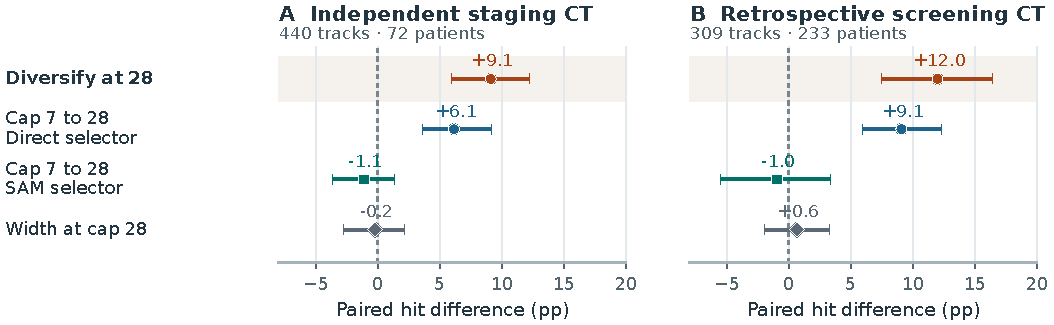
\includegraphics[width=.96\textwidth]{figures/paired_effects.pdf}
\caption{Paired candidate and scorer changes at 3 mm. Points show hit-rate changes in percentage points. Whiskers are paired patient-cluster 95\% intervals. The diversification comparison holds the 28-point count, lattice and scorer fixed. The two cap rows score the same strict lists. The width comparison uses matched support and a cap of 28.}
\label{fig:paired-effects}
\end{figure}

\begin{table}[!ht]
\centering\small
\caption{Point correspondence at 3 mm. Misses are unreachable (U) or reachable but incorrectly selected (R). The full spline maps a single point. Standalone SAM searches the entire common crop.}
\label{tab:point-methods}
\begin{tabular}{lrrrrrrrr}
\toprule
 & \multicolumn{4}{c}{External} & \multicolumn{4}{c}{Screening} \\
\cmidrule(lr){2-5}\cmidrule(lr){6-9}
Route & Avail. & Reach & Hits & Misses (U/R) & Avail. & Reach & Hits & Misses (U/R) \\
\midrule
Original 7 & 345 & 220 & 206 & 220/14 & 285 & 198 & 184 & 111/14 \\
Original 28 + fit & 361 & 248 & 232 & 192/16 & 294 & 229 & 204 & 80/25 \\
Wide relaxed 28 & 381 & 264 & 237 & 176/27 & 301 & 235 & 204 & 74/31 \\
Wide relaxed 28 + Siamese & 381 & 264 & 203 & 176/61 & 301 & 235 & 210 & 74/25 \\
Wide ungated, diversified all & 437 & 348 & 289 & 92/59 & 309 & 289 & 244 & 20/45 \\
Wide raw, all & 437 & 351 & 297 & 89/54 & 309 & 290 & 242 & 19/48 \\
Escalation & 437 & 330 & 280 & 110/50 & 309 & 281 & 240 & 28/41 \\
Standalone SAM & 437 & 396 & 99 & 44/297 & 309 & 308 & 80 & 1/228 \\
Full central Spline & 437 & 243 & 243 & 197/0 & 309 & 211 & 211 & 98/0 \\
\bottomrule
\end{tabular}

\end{table}

\clearpage
\begin{table}[!ht]
\centering\small
\caption{Independent Longitudinal-CT participant flow. The full denominator follows the allocation row.}
\label{tab:external-flow}
\begin{tabular}{lrr}
\toprule
Stage & Patients & Tracks or rows \\
\midrule
Release CSVs & 300 & 4638 \\
Lung annotation rows & 172 & 1488 \\
Clear persistent lung links, single-volume pairs & 107 & 577 \\
Allocated by fixed hash order & 72 & 440 \\
Supported shared crops & 70 & 437 \\
Incomplete shared crop & -- & 3 \\
\bottomrule
\end{tabular}

\end{table}

\begin{table}[!ht]
\centering\small
\setlength{\tabcolsep}{3pt}
\caption{Changes on shared, gained, and lost reach at 3 mm. Shared hits gives first / second on the same tracks. Gain reach gives first-route hits / tracks among newly reachable, and lost reach gives second-route hits / tracks among no longer reachable. Both p90 gives matched available-only error tails in mm.}
\label{tab:reach-transitions}
\begin{tabular}{llrrrrrr}
\toprule
Cohort & First / second & Shared reach & Shared hits & Gain reach & Lost reach & Both avail. & Both p90 \\
\midrule
Screening & Relaxed / original 7 & 194 & 176/181 & 28/41 & 3/4 & 285 & 8.13/7.74 \\
 & Strict 28 / 7, direct & 185 & 172/167 & 23/35 & 0/0 & 292 & 9.28/9.67 \\
 & Strict 28 / 7, SAM & 185 & 104/121 & 14/35 & 0/0 & 292 & 8.72/9.02 \\
 & Original 28 + fit / wide relaxed & 220 & 197/193 & 7/9 & 11/15 & 294 & 8.22/9.20 \\
 & Ungated all / relaxed all & 257 & 225/217 & 19/32 & 0/0 & 301 & 6.57/8.62 \\
\midrule
External & Relaxed / original 7 & 214 & 197/200 & 40/50 & 6/6 & 345 & 10.79/10.48 \\
 & Strict 28 / 7, direct & 202 & 186/192 & 33/39 & 0/0 & 354 & 11.83/12.63 \\
 & Strict 28 / 7, SAM & 202 & 129/144 & 10/39 & 0/0 & 354 & 10.00/11.63 \\
 & Original 28 + fit / wide relaxed & 234 & 221/212 & 11/14 & 25/30 & 361 & 10.67/10.98 \\
 & Ungated all / relaxed all & 300 & 267/264 & 22/48 & 0/0 & 381 & 12.28/11.71 \\
\bottomrule
\end{tabular}

\end{table}

\begin{table}[!ht]
\centering\small
\caption{Frozen current-query error bands, from at most 1.5 mm to 1.5--3 mm to above 3 mm. The top table is screening and the bottom is external. Entries are hits / reach at 3 mm. Query-unavailable tracks are included in the unstratified results.}
\begin{tabular}{lrrr}
\toprule
Route & 194 tracks & 68 tracks & 47 tracks \\
\midrule
Original 7 & 142/143 & 36/40 & 6/15 \\
Original 28 + fit & 156/161 & 42/48 & 6/20 \\
Wide strict 7 & 133/137 & 30/34 & 4/14 \\
Wide strict 28 & 155/158 & 36/41 & 4/21 \\
Wide relaxed 28 & 161/166 & 38/46 & 5/23 \\
Wide ungated, diversified all & 178/185 & 57/65 & 9/39 \\
Wide raw, all & 177/186 & 56/65 & 9/39 \\
Wide relaxed 28 + Siamese & 160/166 & 42/46 & 8/23 \\
Standalone SAM & 62/193 & 14/68 & 4/47 \\
Full central Spline & 157/157 & 46/46 & 8/8 \\
\bottomrule
\end{tabular}
\par\medskip
\begin{tabular}{lrrr}
\toprule
Route & 322 tracks & 72 tracks & 43 tracks \\
\midrule
Original 7 & 175/180 & 27/30 & 4/10 \\
Original 28 + fit & 195/200 & 31/35 & 6/13 \\
Wide strict 7 & 167/169 & 21/25 & 4/8 \\
Wide strict 28 & 192/201 & 21/29 & 6/11 \\
Wide relaxed 28 & 208/218 & 23/34 & 6/12 \\
Wide ungated, diversified all & 238/257 & 39/59 & 12/32 \\
Wide raw, all & 238/259 & 45/59 & 14/33 \\
Wide relaxed 28 + Siamese & 174/218 & 22/34 & 7/12 \\
Standalone SAM & 82/291 & 16/66 & 1/39 \\
Full central spline & 205/205 & 35/35 & 3/3 \\
\bottomrule
\end{tabular}

\end{table}

\begin{table}[!ht]
\centering\small
\caption{Diagnostic rerun on the retrospective cohort with the annotated current point in the same fixed crop. Entries are hits / reach at 3 mm.}
\begin{tabular}{lrr}
\toprule
Route & Frozen query & Current mark \\
\midrule
Original 7 & 184/198 & 211/222 \\
Original 28 + fit & 204/229 & 237/251 \\
Wide strict 28 & 195/220 & 216/241 \\
Wide relaxed 28 & 204/235 & 229/253 \\
Wide ungated, diversified all & 244/289 & 243/293 \\
Full central Spline & 211/211 & 239/239 \\
\bottomrule
\end{tabular}

\end{table}

\begin{table}[!ht]
\centering\small
\caption{External sensitivity using native baseline millimeters, with all 440 tracks in the denominator.}
\begin{tabular}{lrrrrrr}
\toprule
Route & Hit 2 & Hit 3 & Hit 4 & Reach 2 & Reach 3 & Reach 4 \\
\midrule
Original 7 & 149 & 204 & 232 & 163 & 218 & 242 \\
Original 28 + fit & 184 & 230 & 257 & 205 & 245 & 275 \\
Wide strict 7 & 126 & 190 & 218 & 141 & 199 & 232 \\
Wide strict 28 & 159 & 217 & 246 & 185 & 239 & 268 \\
Wide relaxed 28 & 186 & 236 & 264 & 217 & 262 & 295 \\
Wide ungated, diversified all & 254 & 292 & 305 & 335 & 349 & 358 \\
Wide raw, all & 276 & 298 & 310 & 343 & 352 & 360 \\
Wide relaxed 28 + Siamese & 127 & 204 & 253 & 217 & 262 & 295 \\
Full central spline & 197 & 242 & 267 & 197 & 242 & 267 \\
\bottomrule
\end{tabular}

\end{table}

\clearpage
\begin{table}[!ht]
\centering\small
\setlength{\tabcolsep}{4pt}
\caption{Retrospective screening. Reach and hits use all 309 tracks at 2/3/4 mm. Off is the number of returned points outside 3 mm. Conditional hits and tails are reported separately.}
\label{tab:point-luna}
\begin{tabular}{lrrrrrrr}
\toprule
Route & Mean $K$ & Avail. & Reach 2/3/4 & Hits 2/3/4 & Off & Hit$\mid$Reach (\%) & p50/90/95 (mm) \\
\midrule
Original 7 & 5.9 & 285 & 152/198/231 & 134/184/215 & 101 & 92.9 & 2.17/7.74/10.48 \\
Original + fit 7 & 6.0 & 294 & 156/206/237 & 137/191/221 & 103 & 92.7 & 2.18/7.76/10.74 \\
Original + fit 14 & 10.6 & 294 & 183/218/244 & 161/200/225 & 94 & 91.7 & 1.81/7.71/11.26 \\
Original 28 + fit & 16.5 & 294 & 192/229/250 & 163/204/227 & 90 & 89.1 & 1.72/8.22/10.74 \\
Original + fit 56 & 22.4 & 294 & 197/233/252 & 165/205/227 & 89 & 88.0 & 1.66/8.22/10.74 \\
Original + fit 112 & 25.3 & 294 & 197/233/253 & 165/205/227 & 89 & 88.0 & 1.66/8.13/10.50 \\
Original + fit all & 25.3 & 294 & 197/233/253 & 165/205/227 & 89 & 88.0 & 1.66/8.13/10.50 \\
Narrow strict 28 & 15.6 & 286 & 181/220/242 & 154/193/217 & 93 & 87.7 & 1.80/8.15/12.22 \\
Wide strict 7 & 6.0 & 292 & 135/185/216 & 122/167/196 & 125 & 90.3 & 2.45/9.67/13.02 \\
Wide strict 14 & 11.0 & 294 & 156/207/235 & 138/183/210 & 111 & 88.4 & 2.19/9.67/13.00 \\
Wide strict 28 & 19.0 & 294 & 177/220/241 & 151/195/215 & 99 & 88.6 & 1.88/9.39/12.70 \\
Wide strict 56 & 29.7 & 294 & 187/227/247 & 157/198/218 & 96 & 87.2 & 1.80/9.29/12.70 \\
Wide strict 112 & 44.6 & 294 & 194/229/250 & 161/199/220 & 95 & 86.9 & 1.76/9.39/13.66 \\
Wide strict all & 66.8 & 294 & 198/229/251 & 161/198/220 & 96 & 86.5 & 1.75/9.39/12.42 \\
Wide relaxed 7 & 6.8 & 301 & 140/189/219 & 123/170/196 & 131 & 89.9 & 2.49/11.53/13.39 \\
Wide relaxed 14 & 13.3 & 301 & 166/218/244 & 142/189/214 & 112 & 86.7 & 2.20/10.50/13.17 \\
Wide relaxed 28 & 25.1 & 301 & 194/235/252 & 160/204/224 & 97 & 86.8 & 1.81/9.67/13.17 \\
Wide relaxed 56 & 44.8 & 301 & 211/248/260 & 172/210/228 & 91 & 84.7 & 1.68/9.40/12.43 \\
Wide relaxed 112 & 74.9 & 301 & 224/253/265 & 178/215/234 & 86 & 85.0 & 1.63/9.26/12.44 \\
Wide relaxed, all & 128.7 & 301 & 231/257/267 & 179/217/236 & 84 & 84.4 & 1.58/8.62/12.34 \\
Wide relaxed, undiversified all & 1736.1 & 301 & 252/261/270 & 187/224/237 & 77 & 85.8 & 1.36/9.26/12.77 \\
Wide relaxed, undiversified 28 & 27.2 & 301 & 160/189/216 & 141/175/196 & 126 & 92.6 & 2.21/11.43/13.66 \\
Wide ungated 7 & 7.0 & 309 & 140/189/221 & 123/170/196 & 139 & 89.9 & 2.57/11.83/14.45 \\
Wide ungated 14 & 14.0 & 309 & 167/219/246 & 143/190/215 & 119 & 86.8 & 2.21/10.55/16.01 \\
Wide ungated 28 & 28.0 & 309 & 197/242/255 & 164/212/230 & 97 & 87.6 & 1.81/10.18/15.22 \\
Wide ungated 56 & 56.0 & 309 & 226/262/269 & 182/223/234 & 86 & 85.1 & 1.65/10.00/13.23 \\
Wide ungated 112 & 112.0 & 309 & 256/271/282 & 197/232/244 & 77 & 85.6 & 1.50/9.18/16.22 \\
Wide ungated, diversified all & 360.4 & 309 & 284/289/292 & 207/244/255 & 65 & 84.4 & 1.46/7.85/12.44 \\
Wide raw, all & 4851.0 & 309 & 286/290/292 & 205/242/253 & 67 & 83.4 & 1.18/7.45/13.18 \\
Wide ungated, undiversified 28 & 28.0 & 309 & 160/189/216 & 141/175/196 & 134 & 92.6 & 2.32/11.57/14.22 \\
Wide strict 28, no absolute fit & 19.5 & 300 & 180/223/244 & 153/197/216 & 103 & 88.3 & 1.89/9.64/13.56 \\
Wide strict 28, no slack & 22.3 & 294 & 188/226/246 & 158/200/221 & 94 & 88.5 & 1.78/9.30/12.70 \\
Wide strict 28, no witness & 20.4 & 298 & 179/225/245 & 153/199/217 & 99 & 88.4 & 1.89/9.84/13.69 \\
Full central spline & 1.0 & 309 & 170/211/231 & 170/211/231 & 98 & 100.0 & 1.70/8.54/13.84 \\
Wide relaxed 28 + Siamese & 25.1 & 301 & 194/235/252 & 155/210/232 & 91 & 89.4 & 1.87/8.70/13.16 \\
Escalation & 238.9 & 309 & 266/281/288 & 201/240/255 & 69 & 85.4 & 1.55/8.02/12.44 \\
\bottomrule
\end{tabular}

\end{table}

\clearpage
\begin{table}[!ht]
\centering\small
\setlength{\tabcolsep}{4pt}
\caption{External staging CT. Reach and hits use all 440 allocated tracks at 2/3/4 mm. Off is the number of returned points outside 3 mm.}
\label{tab:point-external}
\begin{tabular}{lrrrrrrr}
\toprule
Route & Mean $K$ & Avail. & Reach 2/3/4 & Hits 2/3/4 & Off & Hit$\mid$Reach (\%) & p50/90/95 (mm) \\
\midrule
Original 7 & 4.7 & 345 & 166/220/244 & 152/206/233 & 139 & 93.6 & 2.37/10.48/14.78 \\
Original + fit 7 & 5.0 & 359 & 170/226/252 & 155/211/239 & 148 & 93.4 & 2.41/11.08/15.55 \\
Original + fit 14 & 8.7 & 360 & 197/242/271 & 177/226/253 & 134 & 93.4 & 2.02/10.99/16.24 \\
Original 28 + fit & 13.5 & 361 & 207/248/277 & 187/232/258 & 129 & 93.5 & 1.95/10.67/16.80 \\
Original + fit 56 & 19.0 & 362 & 210/251/280 & 189/234/261 & 128 & 93.2 & 1.92/11.05/16.56 \\
Original + fit 112 & 22.2 & 362 & 212/251/281 & 189/234/262 & 128 & 93.2 & 1.92/10.94/16.56 \\
Original + fit all & 22.2 & 362 & 212/251/281 & 189/234/262 & 128 & 93.2 & 1.92/10.94/16.56 \\
Narrow strict 28 & 13.1 & 348 & 192/239/264 & 166/220/245 & 128 & 92.1 & 2.15/11.35/15.35 \\
Wide strict 7 & 5.0 & 354 & 145/202/233 & 132/192/219 & 162 & 95.0 & 2.71/12.63/16.83 \\
Wide strict 14 & 9.0 & 355 & 166/226/250 & 145/208/233 & 147 & 92.0 & 2.54/12.36/17.22 \\
Wide strict 28 & 15.5 & 357 & 192/241/270 & 166/219/248 & 138 & 90.9 & 2.18/12.58/16.17 \\
Wide strict 56 & 24.7 & 358 & 202/255/277 & 173/229/252 & 129 & 89.8 & 2.07/12.56/15.92 \\
Wide strict 112 & 37.2 & 358 & 208/257/278 & 176/230/253 & 128 & 89.5 & 2.03/11.74/15.92 \\
Wide strict all & 58.9 & 358 & 213/259/281 & 180/232/254 & 126 & 89.6 & 1.99/11.63/16.21 \\
Wide relaxed 7 & 6.0 & 381 & 152/210/245 & 138/196/228 & 185 & 93.3 & 2.85/13.07/18.30 \\
Wide relaxed 14 & 11.6 & 381 & 183/241/266 & 160/217/244 & 164 & 90.0 & 2.54/13.19/19.24 \\
Wide relaxed 28 & 21.9 & 381 & 221/264/295 & 192/237/266 & 144 & 89.8 & 1.99/12.66/18.79 \\
Wide relaxed 56 & 38.6 & 381 & 245/287/309 & 211/257/276 & 124 & 89.5 & 1.83/12.70/18.79 \\
Wide relaxed 112 & 64.3 & 381 & 262/293/315 & 221/260/280 & 121 & 88.7 & 1.71/11.71/18.07 \\
Wide relaxed, all & 114.8 & 381 & 272/300/319 & 228/264/282 & 117 & 88.0 & 1.68/11.71/18.79 \\
Wide relaxed, undiversified all & 1519.2 & 381 & 291/308/325 & 253/275/288 & 106 & 89.3 & 1.26/11.50/17.62 \\
Wide relaxed, undiversified 28 & 24.0 & 381 & 173/220/247 & 156/204/234 & 177 & 92.7 & 2.62/13.19/18.95 \\
Wide ungated 7 & 7.0 & 437 & 154/211/248 & 140/197/231 & 240 & 93.4 & 3.52/27.13/232.21 \\
Wide ungated 14 & 13.9 & 437 & 185/246/272 & 162/221/250 & 216 & 89.8 & 2.89/27.75/232.85 \\
Wide ungated 28 & 27.8 & 437 & 228/274/305 & 197/245/275 & 192 & 89.4 & 2.54/27.51/232.85 \\
Wide ungated 56 & 55.6 & 437 & 265/306/325 & 223/270/290 & 167 & 88.2 & 1.97/28.04/232.91 \\
Wide ungated 112 & 111.2 & 437 & 300/322/341 & 241/278/299 & 159 & 86.3 & 1.82/30.34/229.28 \\
Wide ungated, diversified all & 362.9 & 437 & 339/348/359 & 259/289/306 & 148 & 83.0 & 1.68/30.40/229.28 \\
Wide raw, all & 4817.9 & 437 & 345/351/360 & 277/297/311 & 140 & 84.6 & 1.27/29.91/229.06 \\
Wide ungated, undiversified 28 & 27.8 & 437 & 174/221/250 & 157/205/237 & 232 & 92.8 & 3.33/27.99/232.67 \\
Wide strict 28, no absolute fit & 16.4 & 379 & 200/250/281 & 173/225/257 & 154 & 90.0 & 2.37/13.22/17.64 \\
Wide strict 28, no slack & 18.5 & 357 & 202/248/277 & 174/225/254 & 132 & 90.7 & 2.07/12.16/16.14 \\
Wide strict 28, no witness & 17.2 & 366 & 201/246/277 & 174/223/255 & 143 & 90.7 & 2.13/11.60/15.75 \\
Wide relaxed 28 + Siamese & 21.9 & 381 & 221/264/295 & 134/203/253 & 178 & 76.9 & 2.73/12.43/18.59 \\
Full central spline & 1.0 & 437 & 199/243/267 & 199/243/267 & 194 & 100.0 & 2.41/29.26/231.38 \\
Escalation & 271.3 & 437 & 313/330/345 & 248/280/301 & 157 & 84.8 & 1.78/30.40/229.28 \\
\bottomrule
\end{tabular}

\end{table}

\clearpage
\begin{table}[!ht]
\centering\small
\setlength{\tabcolsep}{3pt}
\caption{SAM point and candidate crossings in retrospective screening CT. The standalone result uses the whole common crop. SAM field prefixes retain its selected point while adding alternative centers.}
\begin{tabular}{lrrrrrrr}
\toprule
Route & Mean $K$ & Avail. & Reach 2/3/4 & Hits 2/3/4 & Off & Hit$\mid$Reach (\%) & p50/90/95 (mm) \\
\midrule
Narrow strict 28 + SAM & 15.6 & 286 & 181/220/242 & 61/117/177 & 169 & 53.2 & 3.33/7.57/10.27 \\
Standalone SAM & 262144.0 & 309 & 308/308/308 & 27/80/147 & 229 & 26.0 & 4.10/9.68/17.38 \\
Original 28 + fit + SAM & 16.5 & 294 & 192/229/250 & 55/131/194 & 163 & 57.2 & 3.24/7.75/9.27 \\
Original 7 + SAM & 5.9 & 285 & 152/198/231 & 59/129/189 & 156 & 65.2 & 3.19/7.67/9.49 \\
SAM field 112 & 112.0 & 309 & 264/278/283 & 27/80/147 & 229 & 28.8 & 4.10/9.68/17.38 \\
SAM field 14 & 14.0 & 309 & 168/223/259 & 27/80/147 & 229 & 35.9 & 4.10/9.68/17.38 \\
SAM field 28 & 28.0 & 309 & 206/250/267 & 27/80/147 & 229 & 32.0 & 4.10/9.68/17.38 \\
SAM field 56 & 56.0 & 309 & 243/269/277 & 27/80/147 & 229 & 29.7 & 4.10/9.68/17.38 \\
SAM field 7 & 7.0 & 309 & 120/193/242 & 27/80/147 & 229 & 41.5 & 4.10/9.68/17.38 \\
Wide ungated 112 + SAM & 112.0 & 309 & 256/271/282 & 34/104/159 & 205 & 38.4 & 3.90/9.29/12.69 \\
Wide ungated 14 + SAM & 14.0 & 309 & 167/219/246 & 54/119/185 & 190 & 54.3 & 3.53/9.43/15.05 \\
Wide ungated 28 + SAM & 28.0 & 309 & 197/242/255 & 53/117/179 & 192 & 48.3 & 3.54/9.58/14.60 \\
Wide ungated 56 + SAM & 56.0 & 309 & 226/262/269 & 45/109/165 & 200 & 41.6 & 3.79/9.46/13.93 \\
Wide ungated 7 + SAM & 7.0 & 309 & 140/189/221 & 57/122/177 & 187 & 64.6 & 3.47/10.14/15.36 \\
Wide ungated, diversified all + SAM & 360.4 & 309 & 284/289/292 & 28/84/148 & 225 & 29.1 & 4.14/8.74/11.98 \\
Wide raw, all + SAM & 4851.0 & 309 & 286/290/292 & 30/80/145 & 229 & 27.6 & 4.10/9.08/12.87 \\
Wide relaxed 28 + SAM & 25.1 & 301 & 194/235/252 & 53/116/175 & 185 & 49.4 & 3.49/9.04/12.36 \\
Wide relaxed 112 + SAM & 74.9 & 301 & 224/253/265 & 40/105/168 & 196 & 41.5 & 3.65/8.36/11.58 \\
Wide relaxed 14 + SAM & 13.3 & 301 & 166/218/244 & 54/119/184 & 182 & 54.6 & 3.47/9.18/12.44 \\
Wide relaxed 56 + SAM & 44.8 & 301 & 211/248/260 & 48/111/167 & 190 & 44.8 & 3.63/8.58/12.41 \\
Wide relaxed 7 + SAM & 6.8 & 301 & 140/189/219 & 57/122/175 & 179 & 64.6 & 3.44/9.63/12.91 \\
Wide relaxed, all + SAM & 128.7 & 301 & 231/257/267 & 36/99/164 & 202 & 38.5 & 3.74/8.36/11.49 \\
Wide relaxed, undiversified 28 + SAM & 27.2 & 301 & 160/189/216 & 72/127/184 & 174 & 67.2 & 3.34/9.84/12.91 \\
Wide strict 112 + SAM & 44.6 & 294 & 194/229/250 & 56/112/171 & 182 & 48.9 & 3.56/8.72/11.92 \\
Wide strict 14 + SAM & 11.0 & 294 & 156/207/235 & 60/118/182 & 176 & 57.0 & 3.44/8.98/12.42 \\
Wide strict 28 + SAM & 19.0 & 294 & 177/220/241 & 61/118/172 & 176 & 53.6 & 3.44/8.98/11.98 \\
Wide strict 56 + SAM & 29.7 & 294 & 187/227/247 & 59/114/168 & 180 & 50.2 & 3.57/8.80/12.49 \\
Wide strict 7 + SAM & 6.0 & 292 & 135/185/216 & 59/121/176 & 171 & 65.4 & 3.34/9.02/12.41 \\
Wide strict all + SAM & 66.8 & 294 & 198/229/251 & 54/109/168 & 185 & 47.6 & 3.57/8.72/11.64 \\
\bottomrule
\end{tabular}

\end{table}

\clearpage
\begin{table}[!ht]
\centering\small
\setlength{\tabcolsep}{3pt}
\caption{SAM point and candidate crossings in external staging CT. Unavailable crops count as misses throughout.}
\begin{tabular}{lrrrrrrr}
\toprule
Route & Mean $K$ & Avail. & Reach 2/3/4 & Hits 2/3/4 & Off & Hit$\mid$Reach (\%) & p50/90/95 (mm) \\
\midrule
Narrow strict 28 + SAM & 13.1 & 348 & 192/239/264 & 84/140/201 & 208 & 58.6 & 3.57/9.48/13.77 \\
Standalone SAM & 260356.7 & 437 & 396/396/397 & 36/99/184 & 338 & 25.0 & 4.37/33.45/230.73 \\
Original 28 + fit + SAM & 13.5 & 361 & 207/248/277 & 68/135/209 & 226 & 54.4 & 3.58/8.90/14.47 \\
Original 7 + SAM & 4.7 & 345 & 166/220/244 & 76/146/201 & 199 & 66.4 & 3.52/8.86/13.61 \\
SAM field 112 & 111.2 & 437 & 330/354/364 & 36/99/184 & 338 & 28.0 & 4.37/33.45/230.73 \\
SAM field 14 & 13.9 & 437 & 204/284/318 & 36/99/184 & 338 & 34.9 & 4.37/33.45/230.73 \\
SAM field 28 & 27.8 & 437 & 268/314/336 & 36/99/184 & 338 & 31.5 & 4.37/33.45/230.73 \\
SAM field 56 & 55.6 & 437 & 302/342/351 & 36/99/184 & 338 & 28.9 & 4.37/33.45/230.73 \\
SAM field 7 & 7.0 & 437 & 152/244/301 & 36/99/184 & 338 & 40.6 & 4.37/33.45/230.73 \\
Wide ungated 112 + SAM & 111.2 & 437 & 300/322/341 & 51/118/204 & 319 & 36.6 & 4.24/26.83/234.58 \\
Wide ungated 14 + SAM & 13.9 & 437 & 185/246/272 & 78/148/202 & 289 & 60.2 & 4.26/25.18/231.38 \\
Wide ungated 28 + SAM & 27.8 & 437 & 228/274/305 & 73/128/198 & 309 & 46.7 & 4.24/26.78/233.14 \\
Wide ungated 56 + SAM & 55.6 & 437 & 265/306/325 & 69/134/209 & 303 & 43.8 & 4.15/26.28/233.75 \\
Wide ungated 7 + SAM & 7.0 & 437 & 154/211/248 & 79/149/197 & 288 & 70.6 & 4.56/25.18/230.99 \\
Wide ungated, diversified all + SAM & 362.9 & 437 & 339/348/359 & 46/97/184 & 340 & 27.9 & 4.42/27.41/228.26 \\
Wide raw, all + SAM & 4817.9 & 437 & 345/351/360 & 40/103/180 & 334 & 29.3 & 4.46/27.59/228.36 \\
Wide relaxed 28 + SAM & 21.9 & 381 & 221/264/295 & 74/134/202 & 247 & 50.8 & 3.81/10.61/16.96 \\
Wide relaxed 112 + SAM & 64.3 & 381 & 262/293/315 & 62/130/207 & 251 & 44.4 & 3.76/10.75/16.51 \\
Wide relaxed 14 + SAM & 11.6 & 381 & 183/241/266 & 78/147/201 & 234 & 61.0 & 3.77/10.90/19.11 \\
Wide relaxed 56 + SAM & 38.6 & 381 & 245/287/309 & 72/143/214 & 238 & 49.8 & 3.69/10.38/16.51 \\
Wide relaxed 7 + SAM & 6.0 & 381 & 152/210/245 & 79/150/196 & 231 & 71.4 & 3.82/12.20/19.43 \\
Wide relaxed, all + SAM & 114.8 & 381 & 272/300/319 & 60/125/205 & 256 & 41.7 & 3.81/10.72/16.96 \\
Wide relaxed, undiversified 28 + SAM & 24.0 & 381 & 173/220/247 & 96/161/207 & 220 & 73.2 & 3.68/12.60/19.46 \\
Wide strict 112 + SAM & 37.2 & 358 & 208/257/278 & 81/139/199 & 219 & 54.1 & 3.69/10.21/14.00 \\
Wide strict 14 + SAM & 9.0 & 355 & 166/226/250 & 81/146/194 & 209 & 64.6 & 3.68/10.41/14.97 \\
Wide strict 28 + SAM & 15.5 & 357 & 192/241/270 & 81/139/196 & 218 & 57.7 & 3.70/10.21/13.34 \\
Wide strict 56 + SAM & 24.7 & 358 & 202/255/277 & 84/146/204 & 212 & 57.3 & 3.58/10.18/13.52 \\
Wide strict 7 + SAM & 5.0 & 354 & 145/202/233 & 80/144/187 & 210 & 71.3 & 3.74/11.63/15.64 \\
Wide strict all + SAM & 58.9 & 358 & 213/259/281 & 79/137/200 & 221 & 52.9 & 3.67/10.12/14.75 \\
\bottomrule
\end{tabular}

\end{table}

\begin{table}[!ht]
\centering\small
\caption{Wide relaxed budget sweep with the frozen Siamese on identical centers. The external sweep is a secondary transfer diagnostic.}
\begin{tabular}{lrrrr}
\toprule
Wide relaxed cap & External hits 2/3/4 & Reach 3 & Screening hits 2/3/4 & Reach 3 \\
\midrule
7 & 108/169/216 & 210 & 122/169/202 & 189 \\
14 & 118/189/235 & 241 & 137/194/221 & 218 \\
28 & 134/203/253 & 264 & 155/210/232 & 235 \\
56 & 136/214/256 & 287 & 166/224/241 & 248 \\
112 & 139/214/262 & 293 & 166/223/241 & 253 \\
all & 140/210/258 & 300 & 167/223/242 & 257 \\
\bottomrule
\end{tabular}

\end{table}

\clearpage
\begin{table}[!ht]
\centering\small
\setlength{\tabcolsep}{4pt}
\caption{Screening timing. Each entry gives median / p90 seconds. Prepared-crop results use 32 queries. The native replay uses eight pairs, four with two measured queries. The four-query column estimates amortization.}
\label{tab:timing-v6}
\begin{tabular}{lrrrrrr}
\toprule
Route & Local & Propose & Score & Native, one & Native, two & Native, four est. \\
\midrule
Original 7 & 0.076/0.083 & 0.039/0.044 & 0.037/0.039 & 29.232/43.329 & 14.768/17.737 & 7.529/11.056 \\
Original 28 + fit & 0.080/0.085 & 0.039/0.042 & 0.041/0.046 & 29.246/43.336 & 14.775/17.741 & 7.536/11.063 \\
Wide relaxed 28 & 0.113/0.123 & 0.061/0.066 & 0.051/0.061 & 29.291/43.364 & 14.815/17.777 & 7.576/11.092 \\
Wide ungated, diversified all & 0.185/0.190 & 0.111/0.115 & 0.074/0.075 & 29.362/43.440 & 14.883/17.845 & 7.645/11.167 \\
Wide raw, all & 0.256/0.262 & 0.057/0.063 & 0.198/0.202 & 29.426/43.512 & 14.951/17.917 & 7.712/11.239 \\
Escalation & 0.253/0.267 & 0.142/0.151 & 0.107/0.117 & 29.340/43.344 & 14.914/17.840 & 7.676/11.071 \\
Full central spline & 3.866/4.693 & 0.039/0.042 & 0.000/0.000 & 32.867/47.038 & 19.382/22.038 & 12.207/14.558 \\
Wide relaxed 28 + Siamese & 0.082/0.088 & 0.060/0.067 & 0.022/0.023 & 29.246/43.337 & 14.776/17.743 & 7.538/11.064 \\
Standalone SAM & 0.033/0.035 & 0.000/0.000 & 0.033/0.035 & 29.201/43.291 & 14.723/17.680 & 7.484/11.018 \\
Wide strict 28 + SAM & 0.090/0.100 & 0.061/0.065 & 0.033/0.036 & 29.265/43.360 & 14.787/17.748 & 7.549/11.087 \\
\bottomrule
\end{tabular}

\end{table}

\begin{table}[!ht]
\centering\small
\caption{External prepared-crop timing on 24 supported patient pairs, one query per pair. Each entry gives median / p90 seconds.}
\begin{tabular}{lrrrr}
\toprule
Route & Local & Propose & Score & Optimize \\
\midrule
Original 7 & 0.075/0.083 & 0.040/0.045 & 0.035/0.042 & 0.000/0.000 \\
Original 28 + fit & 0.084/0.090 & 0.042/0.047 & 0.042/0.046 & 0.000/0.000 \\
Wide relaxed 28 & 0.265/0.539 & 0.223/0.525 & 0.053/0.059 & 0.000/0.000 \\
Wide ungated, diversified all & 0.194/0.458 & 0.120/0.385 & 0.074/0.074 & 0.000/0.000 \\
Wide raw, all & 0.956/1.574 & 0.187/0.442 & 0.692/1.191 & 0.000/0.000 \\
Escalation & 0.284/0.538 & 0.190/0.452 & 0.110/0.120 & 0.000/0.000 \\
Full central Spline & 3.617/4.707 & 0.041/0.046 & 0.000/0.000 & 3.575/4.667 \\
Wide relaxed 28 + Siamese & 0.106/0.424 & 0.077/0.397 & 0.026/0.028 & 0.000/0.000 \\
\bottomrule
\end{tabular}

\end{table}

\begin{table}[!ht]
\centering\small
\setlength{\tabcolsep}{4pt}
\caption{Fixed-budget timing after the accuracy readout. Hit counts use the full staging and screening cohorts. Times are median / p90 seconds of per-query medians from three randomized repetitions on the matched 24 staging and 32 screening workloads. Propose includes residuals, ordering and candidate construction. Score includes descriptor computation and point selection. All replayed counts and selected points equal their saved values.}
\label{tab:fixed-budget-timing}
\begin{tabular}{lrrrrrrrr}
\toprule
Route & Stg. hits & Stg. local & Stg. propose & Stg. score & Scr. hits & Scr. local & Scr. propose & Scr. score \\
\midrule
Fit-only 28 & 205 & 0.098/0.104 & 0.062/0.065 & 0.036/0.041 & 175 & 0.101/0.107 & 0.064/0.066 & 0.036/0.041 \\
Diverse 28 & 245 & 0.120/0.127 & 0.066/0.070 & 0.053/0.059 & 212 & 0.120/0.131 & 0.068/0.070 & 0.051/0.061 \\
Diverse 56 & 270 & 0.131/0.137 & 0.070/0.074 & 0.060/0.065 & 223 & 0.132/0.137 & 0.072/0.074 & 0.060/0.065 \\
Diverse 112 & 278 & 0.142/0.147 & 0.078/0.082 & 0.065/0.067 & 232 & 0.144/0.148 & 0.080/0.082 & 0.065/0.067 \\
Diverse, all & 289 & 0.190/0.199 & 0.116/0.122 & 0.075/0.075 & 244 & 0.190/0.193 & 0.116/0.119 & 0.074/0.074 \\
Exhaustive & 297 & 0.265/0.413 & 0.063/0.068 & 0.201/0.210 & 242 & 0.265/0.267 & 0.064/0.066 & 0.201/0.201 \\
\bottomrule
\end{tabular}

\end{table}

\begin{table}[!ht]
\centering\small
\caption{Out-of-fold development with 145 frozen queries. Geometry uses the direct selector.}
\label{tab:devsearch}
\begin{tabular}{@{}lrrrr@{}}
\toprule
Search & Mean $K$ & Avail. & Reach & Hits \\
\midrule
Original / 7 & 6.0 & 136 & 99 & 94 \\
Original / 14 & 10.2 & 137 & 104 & 97 \\
Original / 28 & 15.6 & 138 & 106 & 96 \\
Original 28 + fit & 16.1 & 140 & 109 & 99 \\
Original 28 + slack & 20.6 & 138 & 110 & 99 \\
Original 28, no witness & 16.8 & 138 & 108 & 98 \\
Narrow 28 (shared) & 16.1 & 141 & 107 & 95 \\
Wide / 7 & 6.2 & 140 & 91 & 83 \\
Wide / 28 & 19.2 & 142 & 105 & 95 \\
Wide relaxed / 28 & 25.5 & 142 & 113 & 100 \\
Anchor affine, screened & 1.4 & 141 & 94 & 93 \\
Anchor affine, open & 1.6 & 145 & 97 & 95 \\
\bottomrule
\end{tabular}

\end{table}

\begin{table}[!ht]
\centering\small
\caption{Native image sampling audit over the timing workloads. Radii are relative to the crop center, mapped back to the current physical frame. Counts refer to queries whose possible raw support reaches the reserved radius or exceeds the native sampling domain.}
\label{tab:native}
\begin{tabular}{@{}llrrrr@{}}
\toprule
Geometry & Scan & Min. mm & Median mm & $\leq10$ mm & Clipped \\
\midrule
Original lattice & current & 18.30 & 18.90 & 0 & 0 \\
Original lattice & prior & 11.32 & 11.75 & 0 & 0 \\
Wide and affine residuals & current & 18.63 & 19.38 & 0 & 0 \\
Wide and affine residuals & prior & 9.41 & 10.15 & 9 & 0 \\
Anchor patches & current & 18.50 & 19.59 & 0 & 0 \\
Anchor patches & prior & 11.05 & 11.93 & 0 & 0 \\
\bottomrule
\end{tabular}

\end{table}

\begin{table}[!ht]
\centering\small
\setlength{\tabcolsep}{4pt}
\caption{Paired training contrasts on identical candidate centers. Entries are percentage-point changes and 95\% paired intervals. Close ranking conditions on tracks with at least one close positive--negative pair.}
\label{tab:learnpairs}
\begin{tabular}{@{}llrrr@{}}
\toprule
Set & First vs. second scorer & $\Delta$ hits & $\Delta$ mixed top-1 & $\Delta$ close ranking \\
\midrule
Original / 7 & Proposals, paired vs. Shell, paired & +2.6 [+0.3, +5.0] & +4.3 [+0.6, +8.2] & +1.5 [-0.3, +3.4] \\
Original / 7 & Proposals, prior only vs. Shell, prior only & -0.3 [-3.2, +2.6] & -0.5 [-5.3, +4.3] & +0.3 [-2.7, +3.5] \\
Original / 7 & Proposals, paired vs. Proposals, prior only & +3.2 [+1.0, +5.7] & +5.3 [+1.5, +9.4] & +2.9 [+0.7, +5.3] \\
Original / 7 & Shell, paired vs. Shell, prior only & +0.3 [-2.6, +3.2] & +0.5 [-4.3, +5.3] & +1.7 [-0.8, +4.8] \\
Original / 7 & Proposals, paired vs. Frozen Siamese & +1.0 [-1.0, +3.1] & +1.6 [-1.8, +5.1] & +0.3 [-1.3, +2.0] \\
Wide relaxed / 28 & Proposals, paired vs. Shell, paired & -1.9 [-4.4, +0.3] & -2.6 [-5.8, +0.4] & +1.5 [+0.2, +3.0] \\
Wide relaxed / 28 & Proposals, prior only vs. Shell, prior only & +0.6 [-2.5, +3.8] & +0.9 [-3.3, +5.0] & +1.9 [-0.2, +4.1] \\
Wide relaxed / 28 & Proposals, paired vs. Proposals, prior only & +1.3 [-1.7, +4.3] & +1.7 [-2.3, +5.7] & +2.4 [+0.8, +4.1] \\
Wide relaxed / 28 & Shell, paired vs. Shell, prior only & +3.9 [+1.6, +6.6] & +5.1 [+2.0, +8.7] & +2.8 [+0.9, +4.9] \\
Wide relaxed / 28 & Proposals, paired vs. Frozen Siamese & -1.6 [-3.8, +0.3] & -2.1 [-5.0, +0.4] & +1.0 [-0.1, +2.3] \\
Wide / 28 & Proposals, paired vs. Shell, paired & -1.3 [-3.3, +0.6] & -1.9 [-4.9, +0.9] & +1.0 [-0.5, +2.6] \\
Wide / 28 & Proposals, prior only vs. Shell, prior only & +0.6 [-1.9, +3.2] & +0.9 [-2.7, +4.7] & +1.6 [-0.7, +4.0] \\
Wide / 28 & Proposals, paired vs. Proposals, prior only & +0.3 [-2.3, +2.9] & +0.5 [-3.4, +4.2] & +1.8 [-0.1, +3.9] \\
Wide / 28 & Shell, paired vs. Shell, prior only & +2.3 [+0.3, +4.6] & +3.3 [+0.5, +6.6] & +2.5 [+0.5, +4.7] \\
Wide / 28 & Proposals, paired vs. Frozen Siamese & -1.0 [-2.7, +0.6] & -1.4 [-4.0, +1.0] & +0.6 [-0.7, +2.0] \\
Anchor affine, screened & Proposals, paired vs. Shell, paired & +0.0 [+0.0, +0.0] & +0.0 [+0.0, +0.0] & +0.0 [+0.0, +0.0] \\
Anchor affine, screened & Proposals, prior only vs. Shell, prior only & -0.6 [-1.6, +0.0] & -5.3 [-13.2, +0.0] & -6.2 [-15.4, +0.0] \\
Anchor affine, screened & Proposals, paired vs. Proposals, prior only & +1.0 [+0.0, +2.2] & +7.9 [+0.0, +17.1] & +9.4 [+0.0, +20.0] \\
Anchor affine, screened & Shell, paired vs. Shell, prior only & +0.3 [-0.7, +1.6] & +2.6 [-6.0, +12.1] & +3.1 [-7.4, +14.3] \\
Anchor affine, screened & Proposals, paired vs. Frozen Siamese & +0.0 [+0.0, +0.0] & +0.0 [+0.0, +0.0] & +0.0 [+0.0, +0.0] \\
Anchor affine, open & Proposals, paired vs. Shell, paired & -0.3 [-1.0, +0.0] & -1.9 [-6.5, +0.0] & -0.9 [-2.9, +0.0] \\
Anchor affine, open & Proposals, prior only vs. Shell, prior only & -1.0 [-2.2, +0.0] & -5.8 [-12.5, +0.0] & -7.0 [-15.0, +0.0] \\
Anchor affine, open & Proposals, paired vs. Proposals, prior only & +1.0 [+0.0, +2.2] & +5.8 [+0.0, +12.9] & +7.9 [+0.0, +17.1] \\
Anchor affine, open & Shell, paired vs. Shell, prior only & +0.3 [-0.7, +1.6] & +1.9 [-4.1, +8.9] & +1.8 [-6.9, +11.4] \\
Anchor affine, open & Proposals, paired vs. Frozen Siamese & -0.3 [-1.0, +0.0] & -1.9 [-6.5, +0.0] & -0.9 [-2.9, +0.0] \\
\bottomrule
\end{tabular}

\end{table}

\clearpage
\begin{figure}[!ht]
\centering
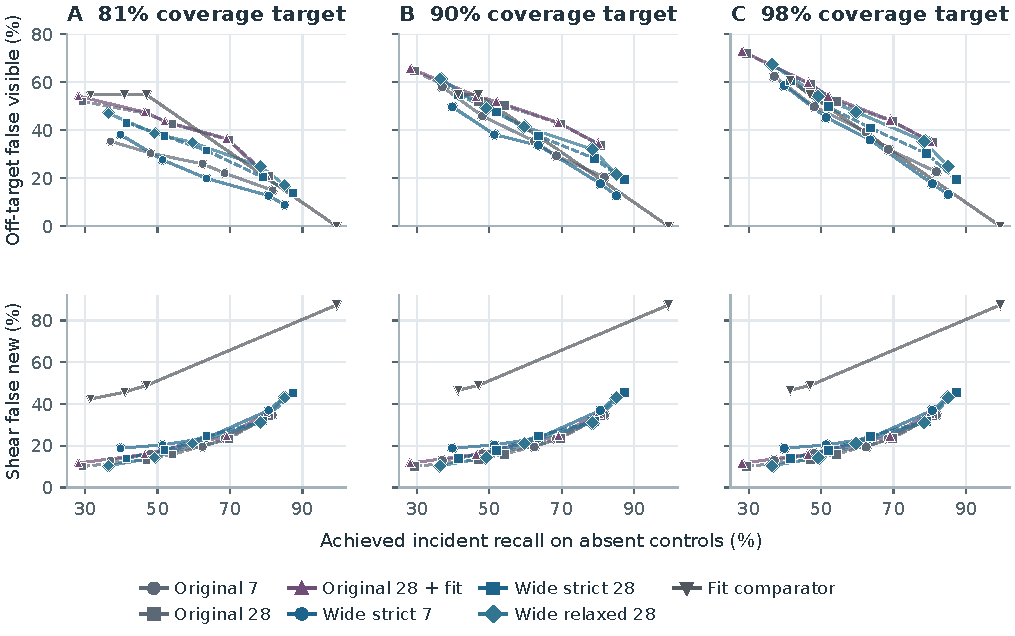
\includegraphics[width=.96\textwidth]{figures/status_achieved.pdf}
\caption{Held-out status tradeoffs at three development coverage targets. The horizontal coordinate is achieved recall on absent controls, not its calibration target. Marker area increases with achieved coverage on absent and standard priors. Lines connect evaluated rules. The matched comparisons additionally require similar class coverage.}
\label{fig:status-achieved}
\end{figure}

\begin{table}[!ht]
\centering\small
\caption{Joint status metrics at the 65\% recall and 81\% coverage target. I and P denote the 181 absent and 181 standard-prior controls. Metrics are percentages of the full applicable denominators, except abstention counts.}
\begin{tabular}{lrrrrrrr}
\toprule
Route & I recall & I false visible & P false new & I coverage & P coverage & Coverage & Abstain \\
\midrule
Original 7 & 62.4 & 22.1 & 5.0 & 84.5 & 90.6 & 87.6 & 45 \\
Original 28 & 54.1 & 26.5 & 5.5 & 80.7 & 85.1 & 82.9 & 62 \\
Original 28 + fit & 51.9 & 29.3 & 4.4 & 81.2 & 86.2 & 83.7 & 59 \\
Wide strict 7 & 63.5 & 18.2 & 10.5 & 81.8 & 88.4 & 85.1 & 54 \\
Wide strict 28 & 63.5 & 21.0 & 16.6 & 84.5 & 84.0 & 84.3 & 57 \\
Wide relaxed 28 & 59.7 & 21.5 & 14.4 & 81.2 & 81.2 & 81.2 & 68 \\
Fit comparator & 47.0 & 52.5 & 0.6 & 99.4 & 99.4 & 99.4 & 2 \\
\bottomrule
\end{tabular}

\end{table}

\clearpage
\begin{table}[!ht]
\centering\small
\caption{New / prior-visible / unresolved on the held-out controls at the 65\% recall and 81\% coverage target. Clean and shear each use 309 tracks. Absent, standard and off-target each use 181.}
\begin{tabular}{lrrrrr}
\toprule
Route & Clean & Shear & Absent & Standard prior & Off-target \\
\midrule
Original 7 & 32/236/41 & 60/187/62 & 113/40/28 & 9/155/17 & 108/47/26 \\
Original 28 & 26/241/42 & 49/202/58 & 98/48/35 & 10/144/27 & 85/77/19 \\
Original 28 + fit & 25/250/34 & 56/214/39 & 94/53/34 & 8/148/25 & 81/79/21 \\
Wide strict 7 & 52/219/38 & 73/183/53 & 115/33/33 & 19/141/21 & 112/36/33 \\
Wide strict 28 & 48/235/26 & 76/195/38 & 115/38/28 & 30/122/29 & 103/57/21 \\
Wide relaxed 28 & 37/245/27 & 65/203/41 & 108/39/34 & 26/121/34 & 95/63/23 \\
Fit comparator & 116/164/29 & 151/119/39 & 85/95/1 & 1/179/1 & 81/99/1 \\
\bottomrule
\end{tabular}

\end{table}

\begin{table}[!ht]
\centering\small
\caption{Status of weak or displaced prior insertions at the same primary target. Entries are new / prior-visible / unresolved on 181 backgrounds per condition.}
\begin{tabular}{lrrrr}
\toprule
Route & Displaced & Small & Faint & Combined \\
\midrule
Original 7 & 79/71/31 & 35/120/26 & 39/112/30 & 106/46/29 \\
Original 28 & 63/82/36 & 33/112/36 & 43/103/35 & 97/54/30 \\
Original 28 + fit & 60/85/36 & 29/115/37 & 37/104/40 & 90/59/32 \\
Wide strict 7 & 76/66/39 & 43/102/36 & 42/96/43 & 110/40/31 \\
Wide strict 28 & 84/73/24 & 60/94/27 & 65/84/32 & 112/44/25 \\
Wide relaxed 28 & 75/78/28 & 53/93/35 & 58/81/42 & 105/42/34 \\
Fit comparator & 22/158/1 & 36/144/1 & 51/129/1 & 76/104/1 \\
\bottomrule
\end{tabular}

\end{table}

\begin{table}[!ht]
\centering\small
\caption{Ranges of paired point estimates across the achieved recall and coverage matches, in percentage points. Each entry compares the first route to the second. Match counts can include identical decisions at distinct calibration targets. The full grid and paired intervals accompany the figures in aggregate form.}
\label{tab:status-matched-v6}
\begin{tabular}{lrrrr}
\toprule
First / second & Matches & Off-target false visible & Shear false new & Off-target coverage \\
\midrule
Wide strict 28 / Wide strict 7 & 23 & +1.7 to +15.5 & -5.2 to +1.9 & -5.0 to +6.6 \\
Wide relaxed 28 / Original 7 & 9 & -0.6 to +12.2 & -2.6 to +1.6 & -3.9 to +5.0 \\
Original 28 + fit / Wide relaxed 28 & 12 & -1.1 to +10.5 & +1.6 to +4.5 & -2.2 to +8.3 \\
Original 28 + fit / Original 7 & 11 & +6.1 to +17.1 & -0.3 to +1.3 & -6.6 to +7.2 \\
Original 28 / Original 7 & 11 & +6.1 to +16.6 & -2.9 to +0.0 & -6.1 to +7.2 \\
Wide relaxed 28 / Fit comparator & 5 & -0.6 to -0.6 & -34.6 to -34.6 & +0.6 to +0.6 \\
\bottomrule
\end{tabular}

\end{table}

\begin{table}[!ht]
\centering\small
\caption{Archived exploratory TCIA status. Inc. is incident-new out of 91. FN and P res. use the 13 prior-visible marks. Res. uses all 104. Sheared scans use the same thresholds fitted to the other folds' clean cases.}
\label{tab:tcia}
\begin{tabular}{lrrrrrrrrrr}
\toprule
 & \multicolumn{5}{c}{Clean} & \multicolumn{5}{c}{Sheared prior} \\
Method & Inc. & FN & Res. & P res. & AUC & Inc. & FN & Res. & P res. & AUC \\
\midrule
Patch / first & 58 & 2 & 87 & 11 & 0.819 & 54 & 4 & 83 & 11 & 0.790 \\
Patch / set & 56 & 4 & 86 & 12 & 0.790 & 54 & 3 & 79 & 10 & 0.779 \\
Direct / first & 61 & 3 & 86 & 12 & 0.803 & 60 & 3 & 81 & 10 & 0.768 \\
Direct / set & 57 & 2 & 85 & 11 & 0.779 & 54 & 2 & 81 & 11 & 0.784 \\
Siamese / set & 59 & 5 & 89 & 12 & 0.751 & 58 & 3 & 84 & 11 & 0.727 \\
Witness-first & 59 & 2 & 87 & 12 & 0.777 & 50 & 1 & 78 & 10 & 0.777 \\
Fit gate, recalibrated & 58 & 3 & 84 & 11 & 0.735 & 60 & 2 & 81 & 10 & 0.790 \\
Fit gate, frozen & 60 & 4 & 84 & 11 & 0.735 & 63 & 4 & 81 & 10 & 0.790 \\
\bottomrule
\end{tabular}

\end{table}

\clearpage
{\small
\bibliographystyle{ieeenat_fullname}
\bibliography{refs}
}
\end{document}
